\documentclass[sans,mathserif]{beamer}
%handout,notes=show

%\usepackage{pgfpages}
%\pgfpagesuselayout{8 on 1}[a4paper,border shrink=5mm]

\usetheme{default}
\usepackage{fp}
\usepackage[thicklines]{cancel}
\usepackage{tikz}
\usepackage{multirow}
\usepackage{amsmath}
\usepackage{ifthen}
\usepackage{animate}
\usepackage{setspace}
\usepackage{forloop}
%\usepackage{concmath}
%\usepackage{pxfonts}
%\usepackage{eulervm}
%\usepackage{mathpazo}
%\renewcommand\mathfamilydefault{\rmdefault}

%\usefonttheme{professionalfonts}
%\setmathfont{}
%\setsansfont{Palatino}
\usetikzlibrary{arrows,backgrounds,positioning,fit,chains,shapes,calc}

%\usepackage{handoutWithNotes}
%\pgfpagesuselayout{4 on 1 with notes}[a4paper,border shrink=5mm]

\setbeamertemplate{navigation symbols}{}

\title{Basics of modern computers}
\author{Dag Sverre Seljebotn}
%\institute{Department of Mathematics \\ University of Oslo}
\date{September 7, 2012}

\newcommand{\V}{\vskip1em}

\setbeamersize{sidebar width left=0cm, sidebar width right=0cm}
\setbeamersize{text margin left=.8cm, text margin right=.8cm}

\defbeamertemplate{note page}{infolines}
{%
  \vskip3em
%  \setstretch{1.8}
  \Large
  \rmfamily
  \insertnote
}
\setbeamertemplate{note page}[infolines]

\renewcommand{\CancelColor}{\color{red}}


\begin{document}


\begin{frame}
  \titlepage
\end{frame}

\begin{frame}

  \begin{center}
    {\Large The world of the 50's to 90's:\\Central Processing Unit + Random Access Memory}
  \end{center}
\end{frame}

% \begin{frame}{Memory, encoding and pointers}
%   \begin{center}
%   von Neumann architecture: CPU $\leftrightarrow$ memory bus $\leftrightarrow$ memory

% ~

%     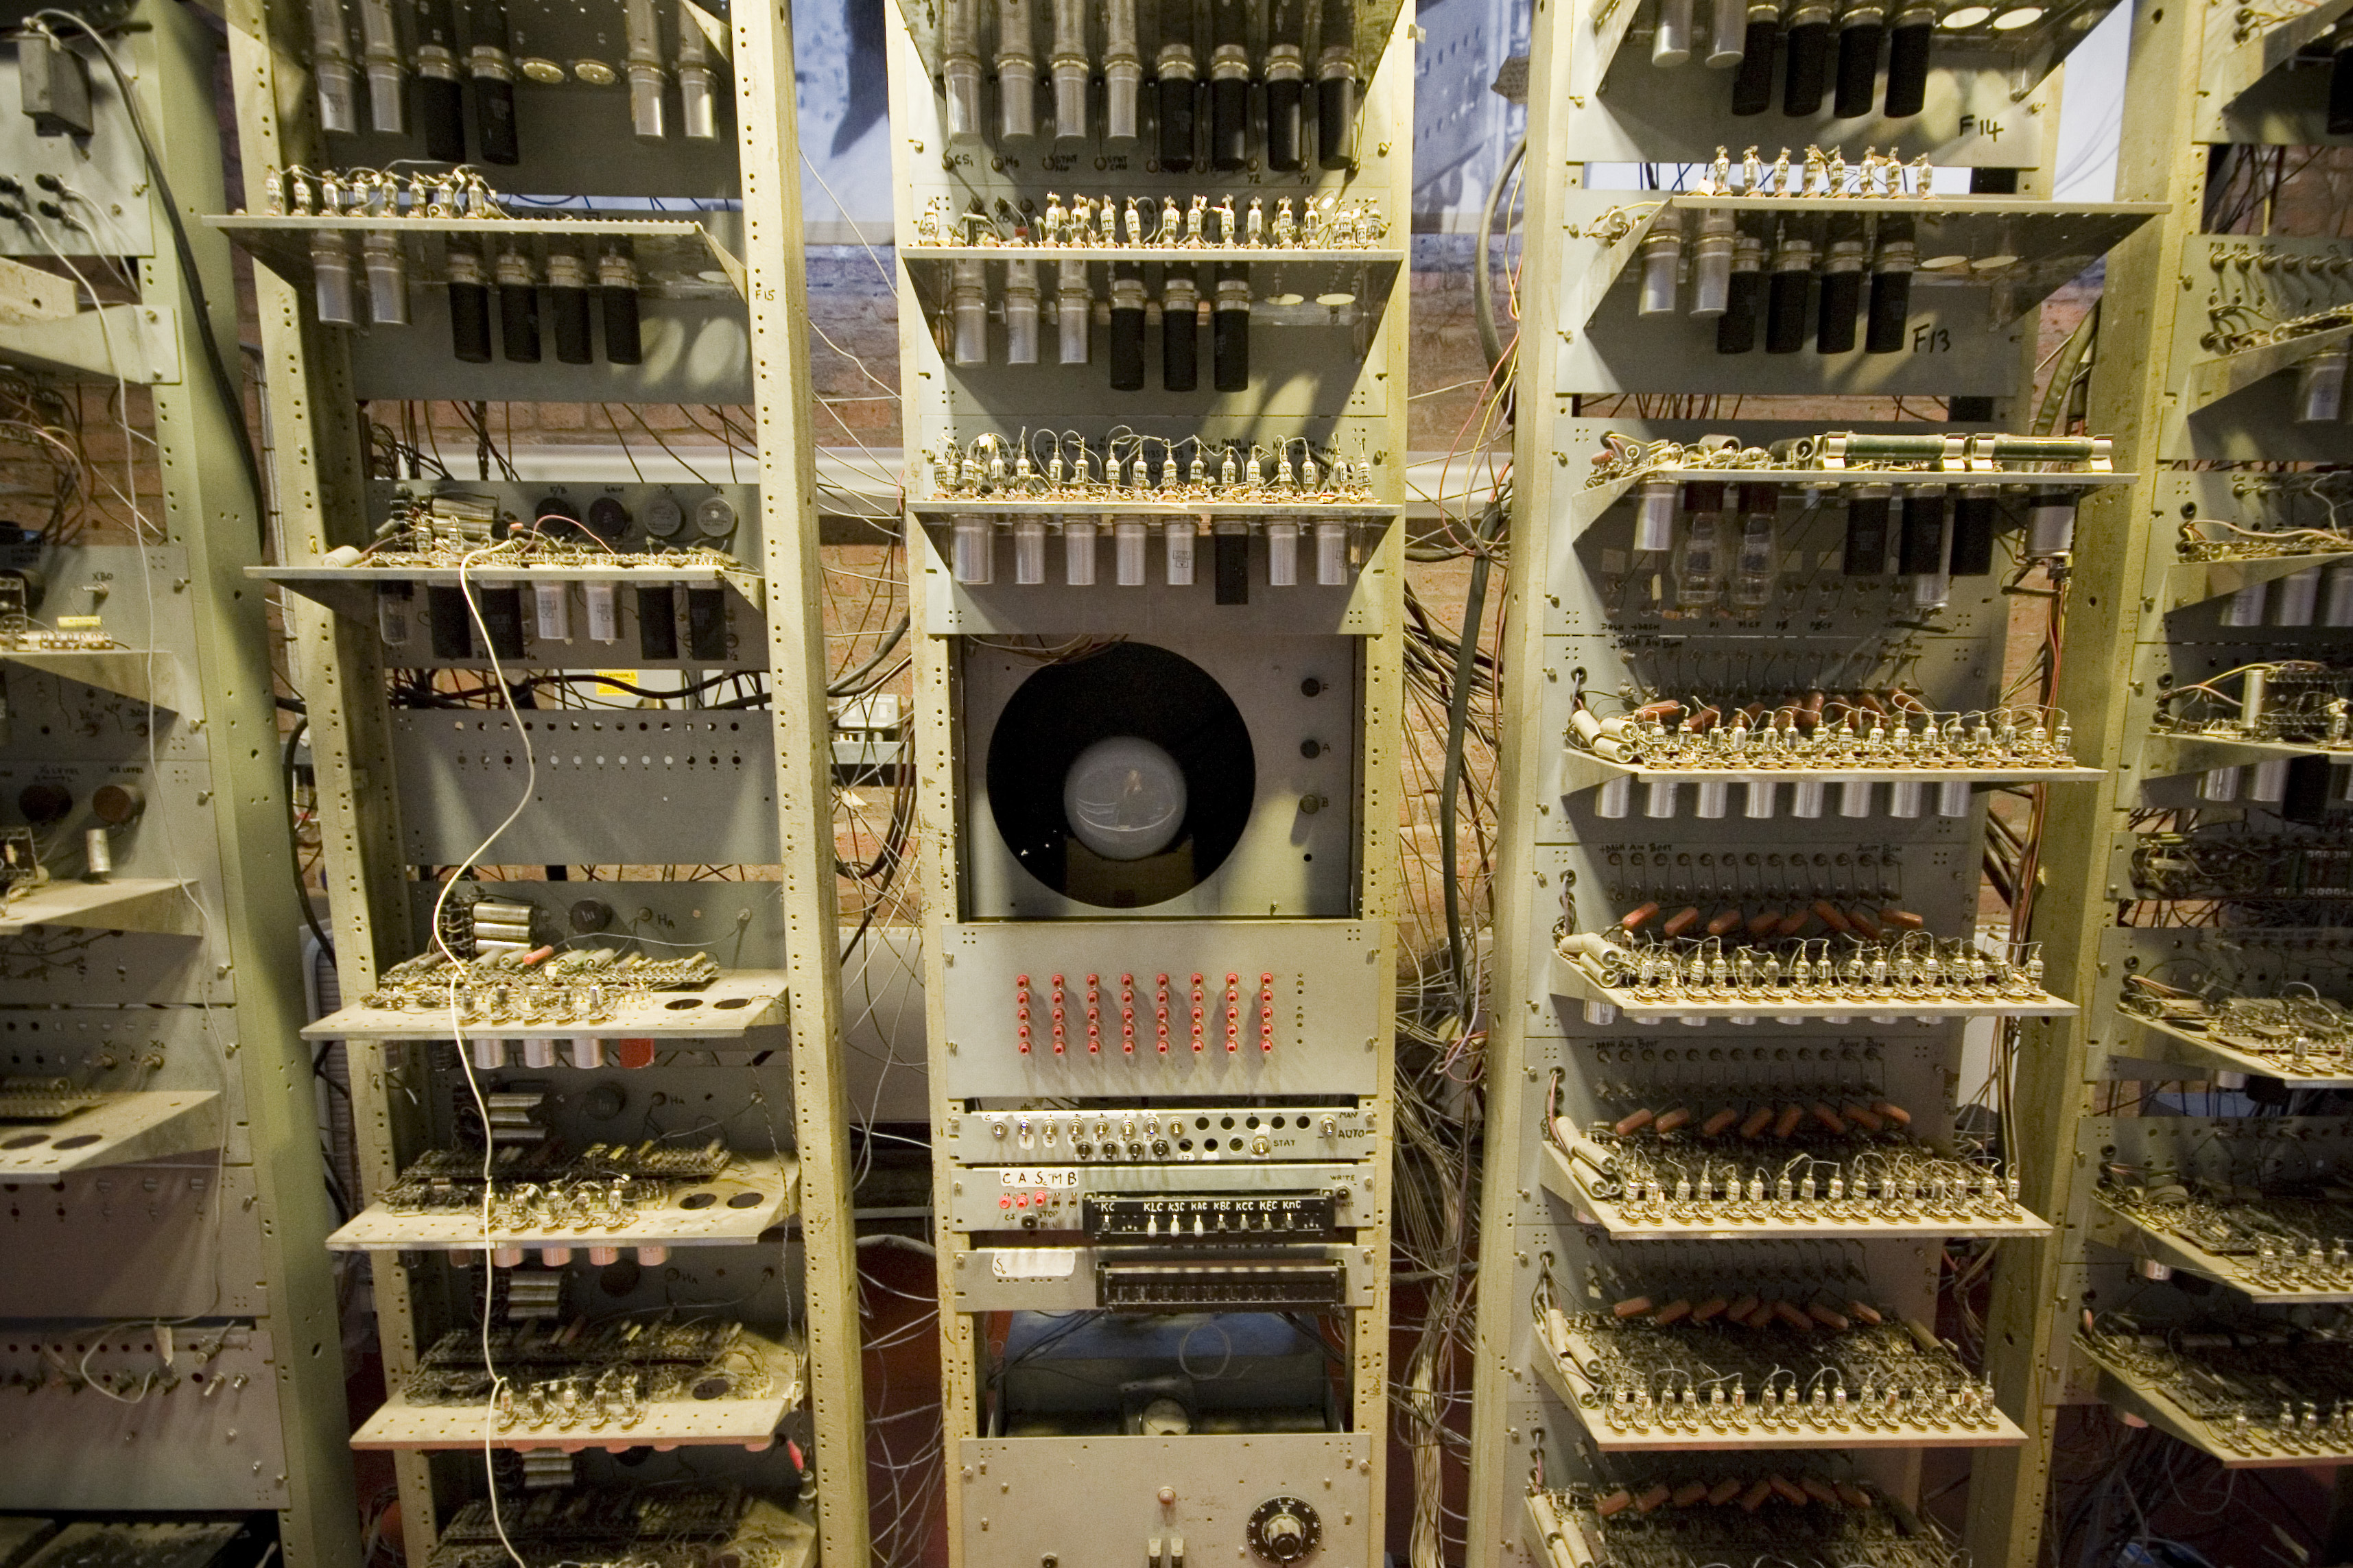
\includegraphics[width=0.7\textwidth]{SSEM.jpg}\\
%     Manchester Small-Scale Experimental Machine, world's first
%     stored-program computer (1948)
%   \end{center}
% \end{frame}

\newcommand{\bs}[3]{{\color{blue}#1} \cdot {#2}^{#3} }
\newcommand{\br}[3]{{\color{red}#1} \cdot {#2}^{#3} }
\begin{frame}{Memory, encoding and pointers}

  Everything (data, program) is encoded in {\em memory bytes},
  which (nowadays) are always 8 bits, allowing $2^8=256$ distinct values.

%124     124    0x7c   |    01111100 
{\small
  \begin{align*}
    124_{10} &= \bs{1}{10}{2} + \bs{2}{10}{1} + \bs{4}{10}{0} \\
    &= \bs{0}{2}{7} + \bs{1}{2}{6} + \bs{1}{2}{5}
              + \bs{1}{2}{4} + 
              \only<1>{\bs{1}{2}{3} + \bs{1}{2}{2} + \bs{0}{2}{1} + \bs{0}{2}{0}}
              \only<2>{\br{1}{2}{3} + \br{1}{2}{2} + \br{0}{2}{1} + \br{0}{2}{0}}
              \\
\uncover<2->{
 &= \bs{7}{16}{1} + \br{12}{16}{0} = \text{\tt 0x7c}}
  \end{align*}
}

  Demo: {\tt binary.c}
\end{frame}

\begin{frame}{Pointers (as seen in C)}
  \begin{tabular}{lll}
    \uncover<+->{{\tt int32\_t x;} & \quad\quad Declare a 4-byte integer ``x'' \\}
    \uncover<+->{{\tt x = 42;} & \quad\quad Memory of ``x'' now contains 42 \\}
    \uncover<+->{{\tt int32\_t *p;} & \quad\quad Declare an 8-byte {\bf pointer to int} ``p'' \\}
    \uncover<+->{{\tt p = \&x;} & \quad\quad Memory of ``p'' now contains 0x00007fffa63cc4b0 \\}
    \uncover<+->{{\tt *p = 10;} & \quad\quad Memory of ``x'' now contains 10 \\}
  \end{tabular}
\end{frame}

\begin{frame}{Pointers and arrays...}
  \begin{tabular}{lll}
    \uncover<+->{{\tt int32\_t *p} & \quad\quad ``x'' is a pointer to integers \\}
    \uncover<+->{{\tt p = malloc(40);} & \quad\quad Allocate space for 10 integers (``array'') \\
     {\tt } & \quad\quad Memory of ``x'' contains 0x00007fffa63cc4b0 \\}
    \uncover<+->{{\tt int32\_t *u;} & \quad\quad  \\}
    \uncover<+->{{\tt u = p + 1;} & \quad\quad Memory of ``u'' contains 0x00007fffa63cc4b4   \\}
    \uncover<+->{{\tt *p = 10;} & \quad\quad Assign first element of array   \\}
    \uncover<+->{{\tt *u = 20;} & \quad\quad Assign second element of array   \\ & \\}

    \uncover<+->{{\tt p[0] = 10;} & \quad\quad Same as {\tt *p = 10} \\ }
    \uncover<+->{{\tt p[1] = 20;} & \quad\quad Same as {\tt *(p + 1) = 20} \\ }
    \uncover<+->{{\tt p[10] = 30;} & \quad\quad Trampling on unallocated memory! \\ }
  \end{tabular}
\end{frame}

\begin{frame}[fragile]{Multi-dimensional arrays}
\begin{verbatim}
int32_t array = malloc(400);
int32_t nrows = 5, ncols = 20;

/* Treat memory in row-major ordering (C-order) */
for (int32_t i = 0; i < nrows; i++) {
  for (int32_t j = 0; j < ncols; j++) {
    array[i * ncols + j] = some_function_of(i, j);
  }
}

/* Treat memory in column-major ordering (Fortran-order) */
for (int32_t i = 0; i < nrows; i++) {
  for (int32_t j = 0; j < ncols; j++) {
    array[i + j * nrows] = some_function_of(i, j);
  }
}
\end{verbatim}
\end{frame}

\begin{frame}[fragile]{Other uses for pointers}
Consider the Fortran routine:
{\color{blue}\begin{verbatim}
subroutine square_me(x)
    integer(4) :: x
    x = x * x
end subroutine
...
call square_me(a) ! a is squared
\end{verbatim}}

~

C is closer to hardware:
{\color{blue}\begin{verbatim}
void square_me(int32_t x) {
    x = x * x;
}
...
square_me(a); /* nothing happens */
\end{verbatim}}

\end{frame}

\begin{frame}[fragile]{Other uses for pointers}
Consider the Fortran routine:
{\color{blue}\begin{verbatim}
subroutine square_me(x)
    integer(4) :: x
    x = x * x
end subroutine
...
call square_me(a) ! a is squared
\end{verbatim}}

~

C is closer to hardware:
{\color{blue}\begin{verbatim}
void square_me(int32_t *p) {
    int32_t x = *p;
    *p = x * x;
}
...
square_me(&a); /* a is squared */
\end{verbatim}}

\end{frame}


\begin{frame}{Simple model of CPUs}
  \begin{itemize}
  \item<+-> {\bf Registers:} ``Hardware variables''. 
    E.g., RAX/EAX, RBX/EAX, XMM0, \dots; about 32 registers on 64-bit
    AMD/Intel CPUs
  \item<+-> {\bf Instructions:} Stream of numbers telling the CPU
    what to do.
    \begin{tabular}{ll}

      \uncover<+->{{\tt mov    eax, [rsp]} & \quad\quad Load from memory \\}
      \uncover<+->{{\tt imul eax, eax} & \quad\quad Do something with register \\}
      \uncover<+->{{\tt mov    [rsp], eax} & \quad\quad Store to memory \\}
    \end{tabular}
\end{itemize}

\uncover<+->{Example: Disassemble {\tt add\_and\_square.o}}

\end{frame}


\begin{frame}{Ways of using memory}

\uncover<+->{Conventionally we divide memory into:}
  \begin{itemize}
  \item<+-> {\bf Static}: Your program, global variables, constants
  \item<+-> {\bf Heap}: Dynamically allocated/deallocated blocks
    \begin{itemize}
    \item C: {\tt malloc()}, {\tt free()} functions
    \item C++: {\tt new}, {\tt delete} keywords
    \item Fortran: {\tt allocate}, {\tt deallocate} keywords
    \item Modern languages: {\tt new} + Garbage Collection
    \end{itemize}
  \item<+-> {\bf Stack}: Allocated at program startup
    \begin{itemize}
    \item Implicitly used through program flow
    \end{itemize}
  \end{itemize}

~

\uncover<4->{Demo program: {\tt knapsack.c} }

\end{frame}

\begin{frame}{Virtual memory}
  \begin{tikzpicture}
    \node at (0,0) {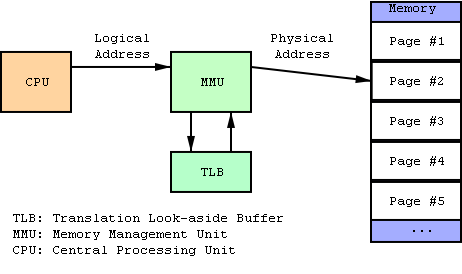
\includegraphics[width=.35\textwidth]{mmu.png}};
    \node at (6,-2) {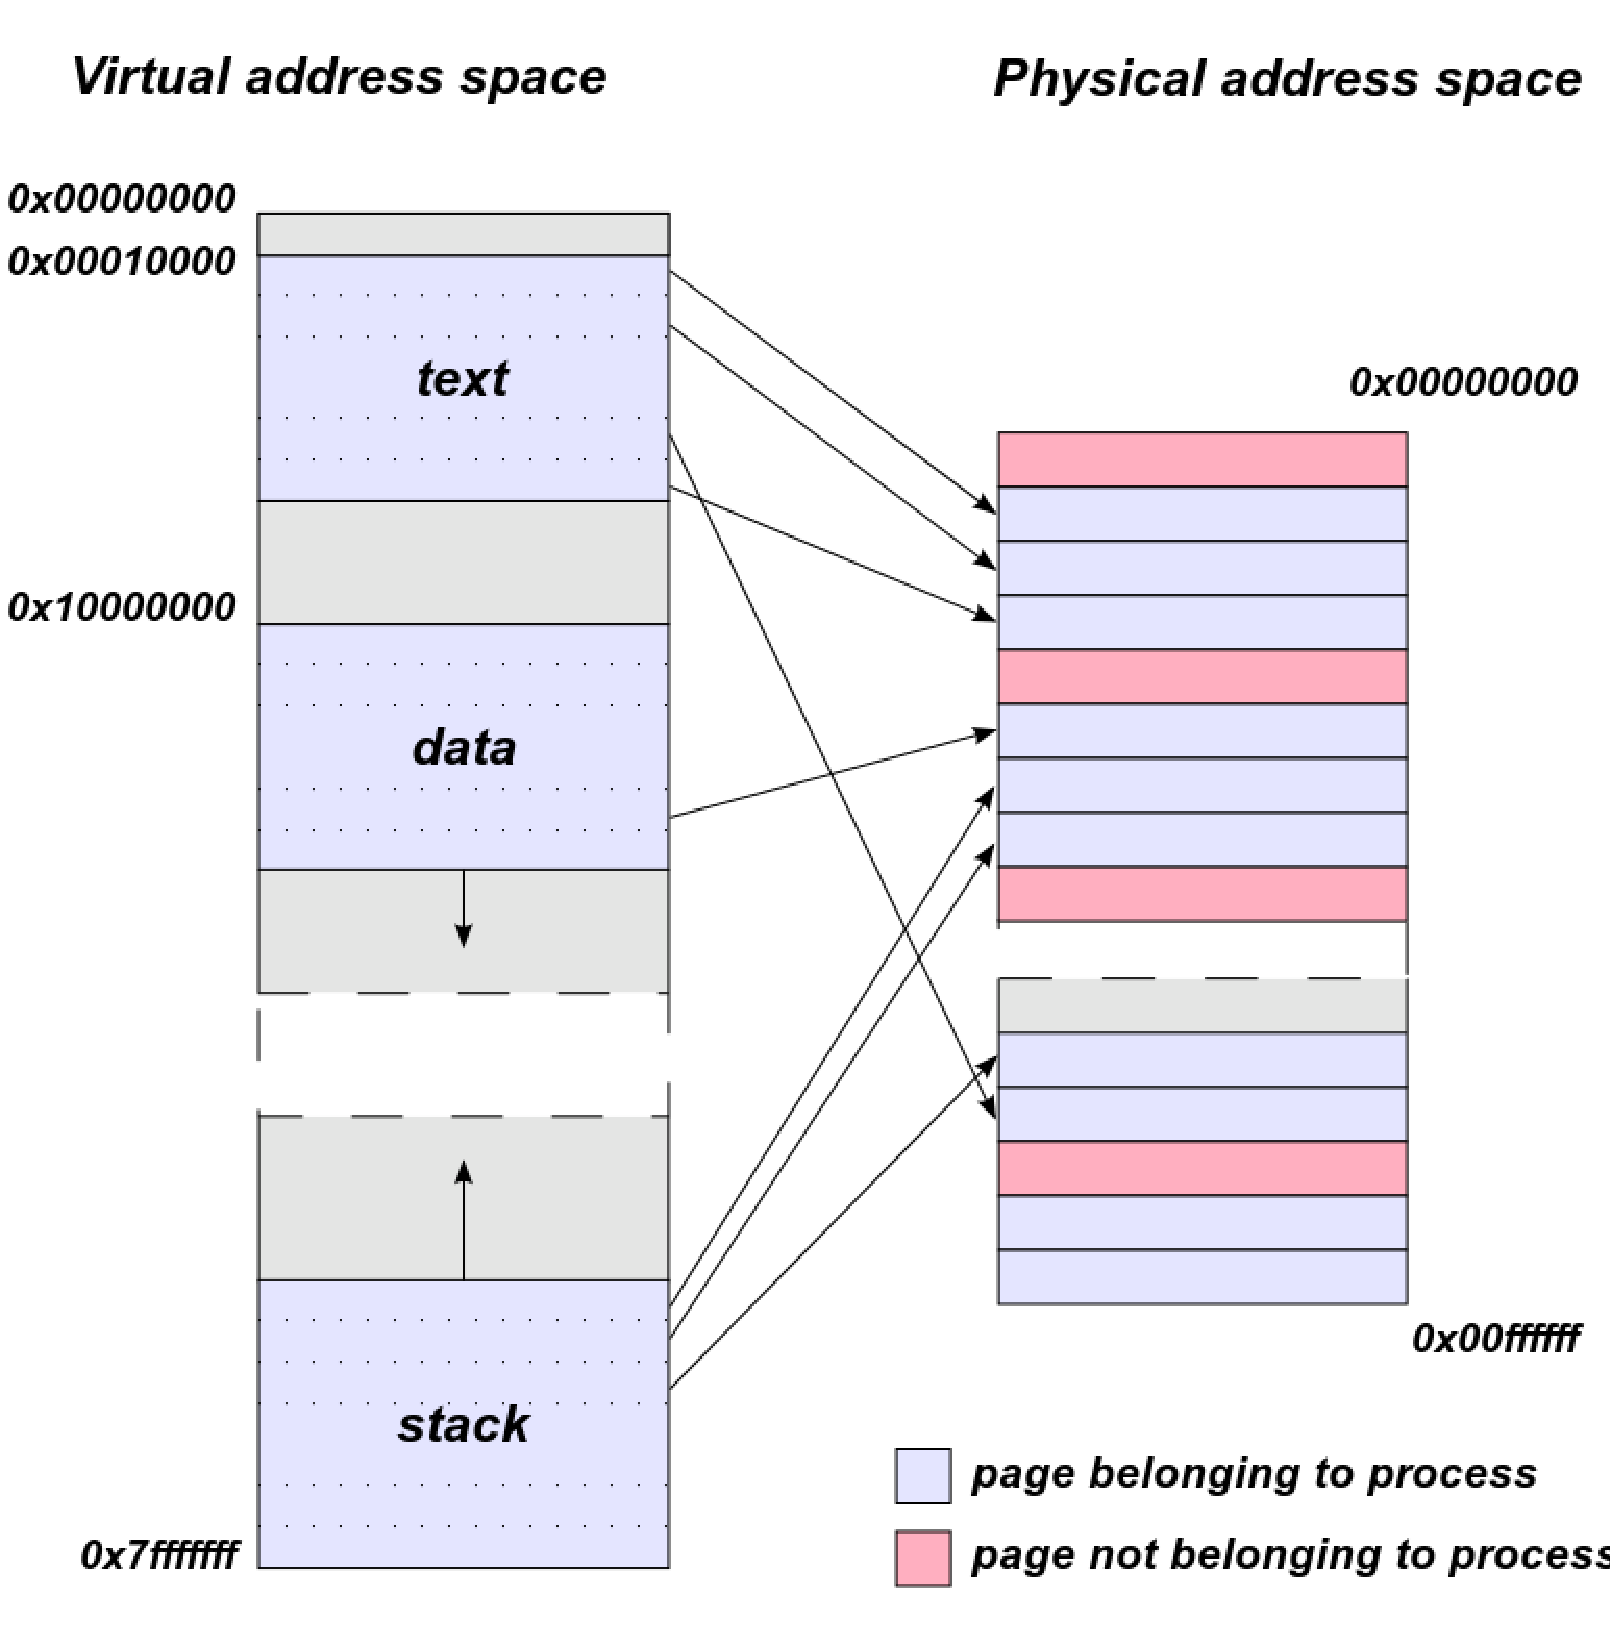
\includegraphics[width=.6\textwidth]{virtualmemory.pdf}};
  \end{tikzpicture}
{\tiny Illustrations from Wikipedia}
\end{frame}


\begin{frame}
  
  \begin{center}
    \Large The memory bandwidth wall
  \end{center}
\end{frame}

\begin{frame}{Benchmarking}

\begin{itemize}
\item<+-> {\bf Problem:} What speed is your CPU {\em really} running at?
  \begin{enumerate}
  \item Power saving
  \item ``Turbo mode''
  \end{enumerate}
\vspace{0.2cm}
\uncover<+->{{\bf Solution:} Disable these features}
\vspace{0.5cm}

\item<+-> {\bf Problem:} Interruptions from the OS\\
\vspace{0.2cm}
\uncover<+->{
  {\bf Solution:} Take many samples of {\em wall time}, then use {\em minimum}. \\
  For each sample, may have to repeat and average.
}
\vspace{0.5cm}

\item<+-> {\bf Problem:} Does benchmark include memory bus etc. or just CPU? \\
\uncover<+->{{\bf Solution:} Benchmark using all CPU cores and with realistically
sized data sets}
\vspace{0.5cm}

\item<+-> {\bf Problem:} The compiler optimizing away the test code

\end{itemize}

\end{frame}

\begin{frame}
Experiments exploring memory bus, cache, cache lines:
\begin{enumerate}
\item<+-> Memory bandwidth
\item<+-> Memory latency
\item<+-> Matrix transpose
\item<+-> OpenMP cache-line ping-pong
\end{enumerate}
\end{frame}

\begin{frame}{Matrix multiplication (Goto \& van de Geijn, 2008)}
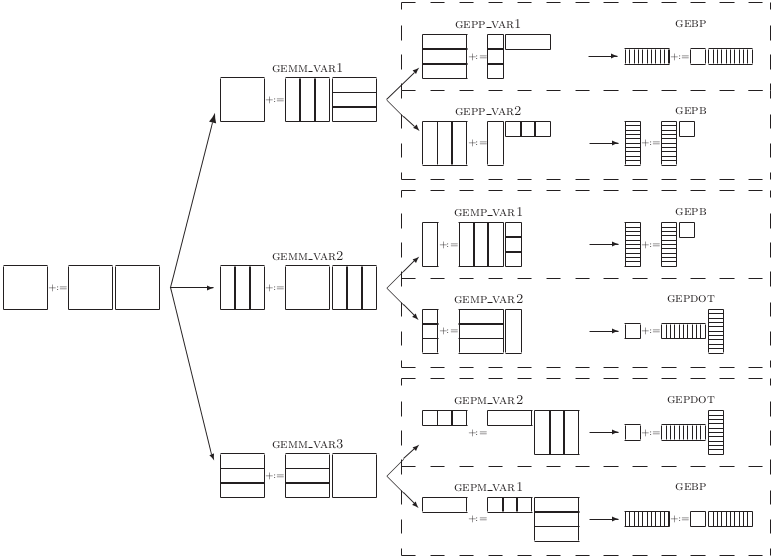
\includegraphics[width=\textwidth]{goto_matmul.png}  
\end{frame}

\begin{frame}
  \begin{center}
    \LARGE A more complicated picture of CPUs
  \end{center}
\end{frame}

\begin{frame}{CPUs getting more complicated}
  \begin{center}
    \only<1>{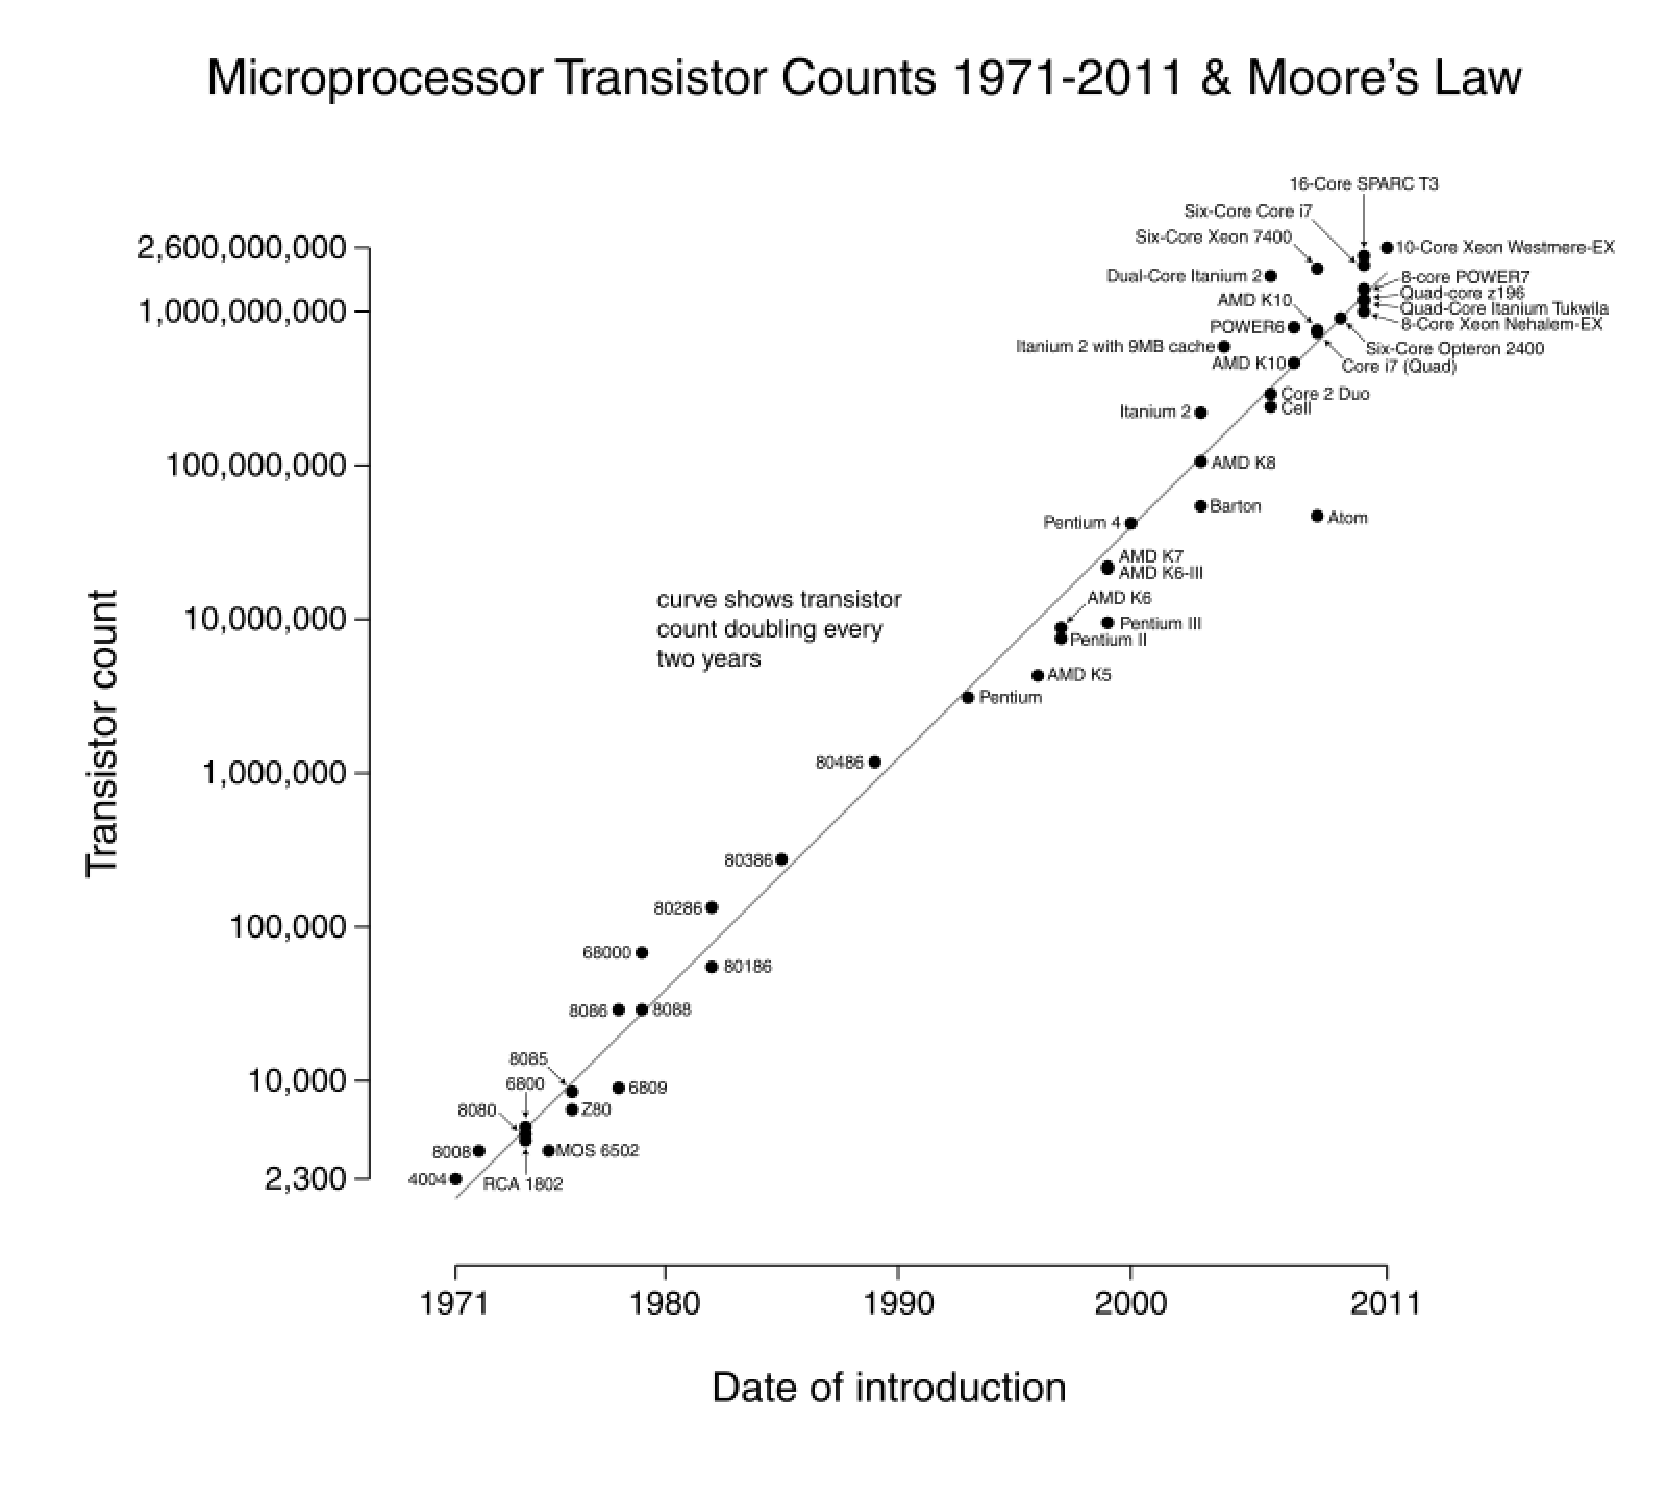
\includegraphics[width=0.8\textwidth]{transistors.pdf}}
    \only<2>{But:\\[5mm]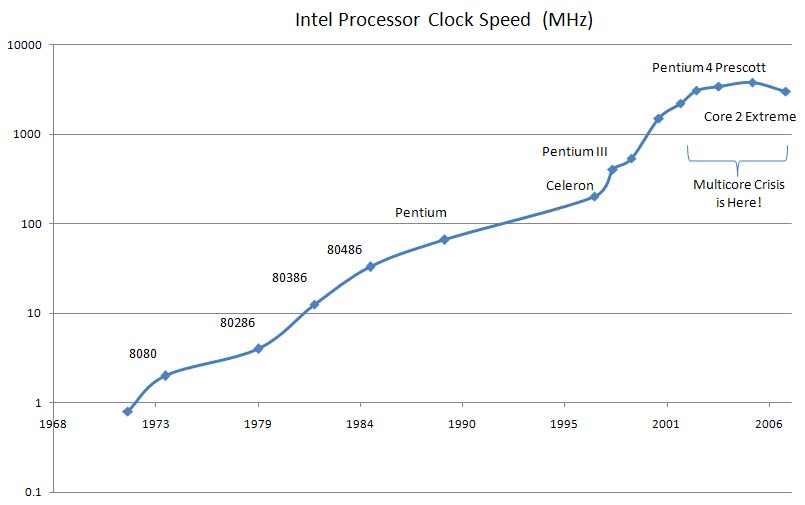
\includegraphics[width=0.8\textwidth]{clockspeeds.jpg}}
  \end{center}
  
\end{frame}

\begin{frame}{CPUs today}
  \begin{center}
    \only<1>{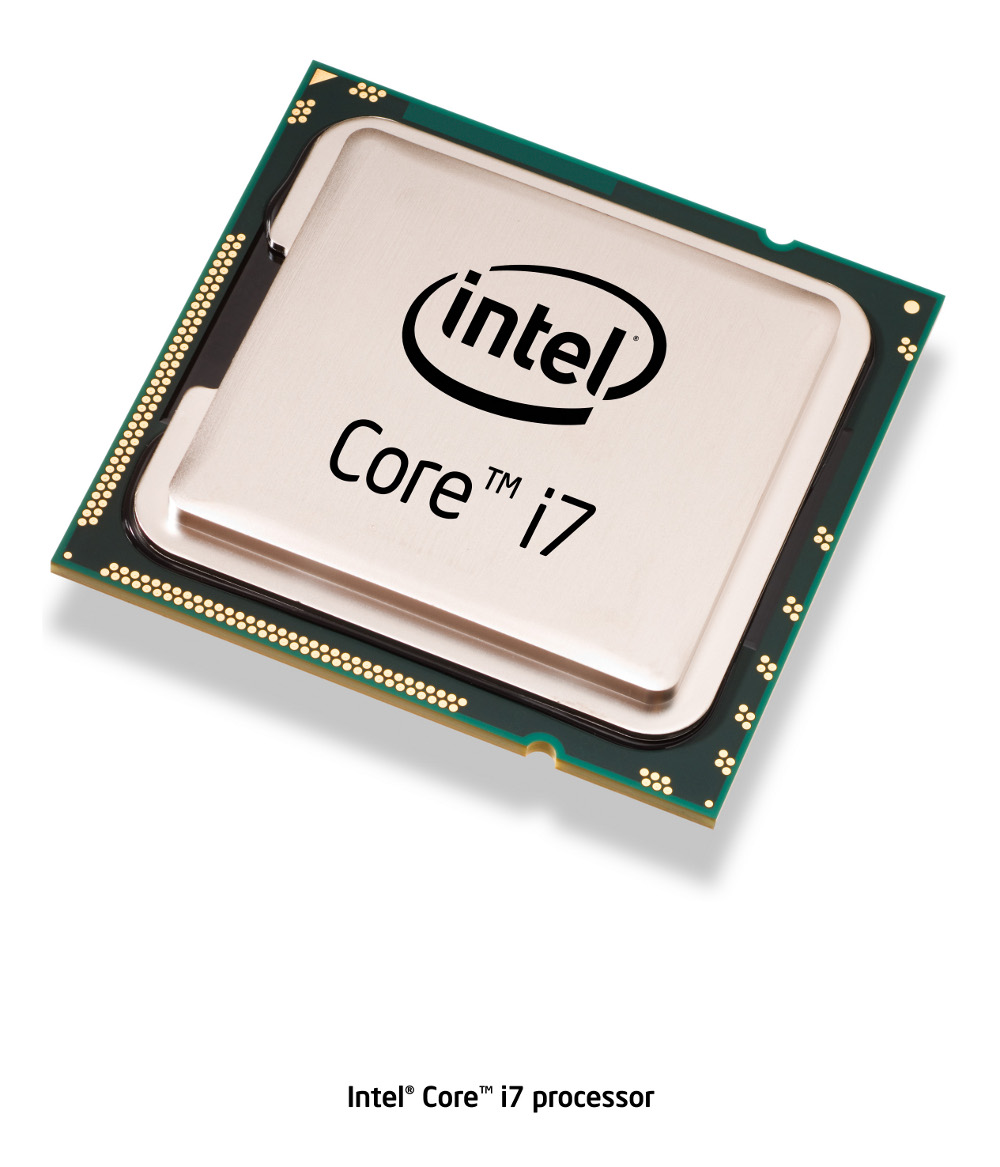
\includegraphics[width=0.8\textwidth]{nehalem_front.jpg}}
    \only<2>{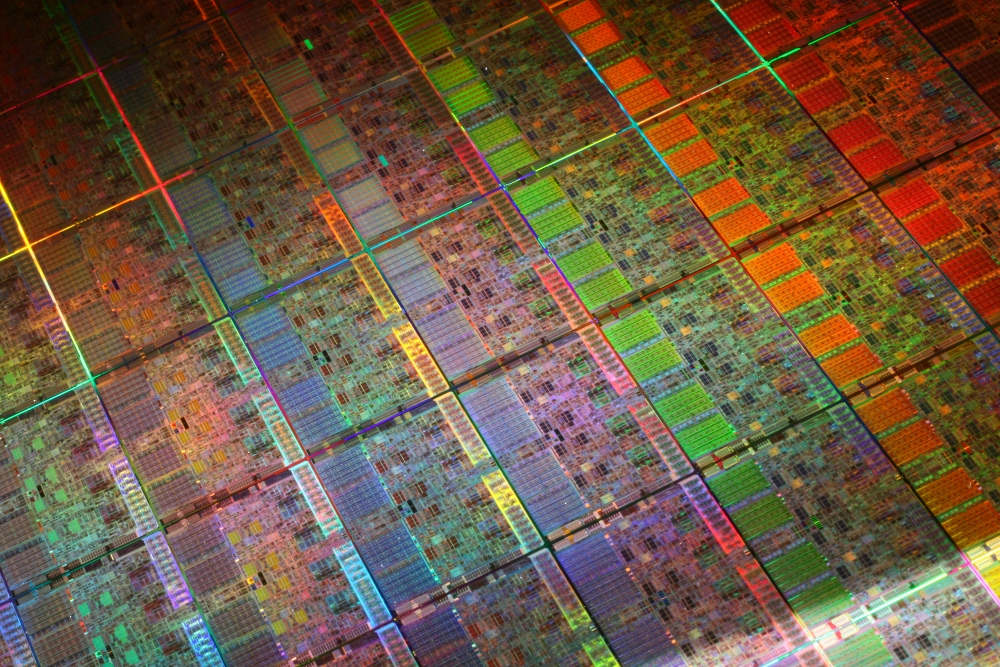
\includegraphics[width=0.8\textwidth]{nehalem_wafer.jpg}}
    \only<3>{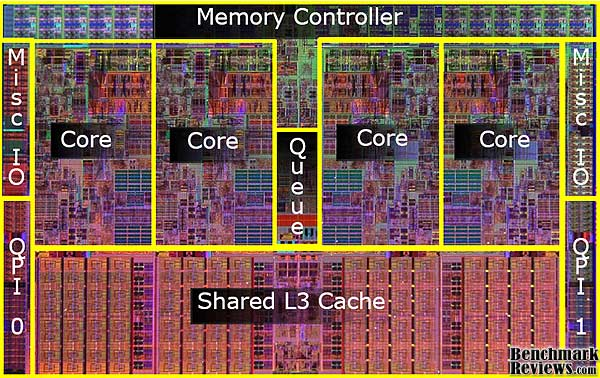
\includegraphics[width=0.8\textwidth]{nehalem_callout.jpg}}
    \only<4>{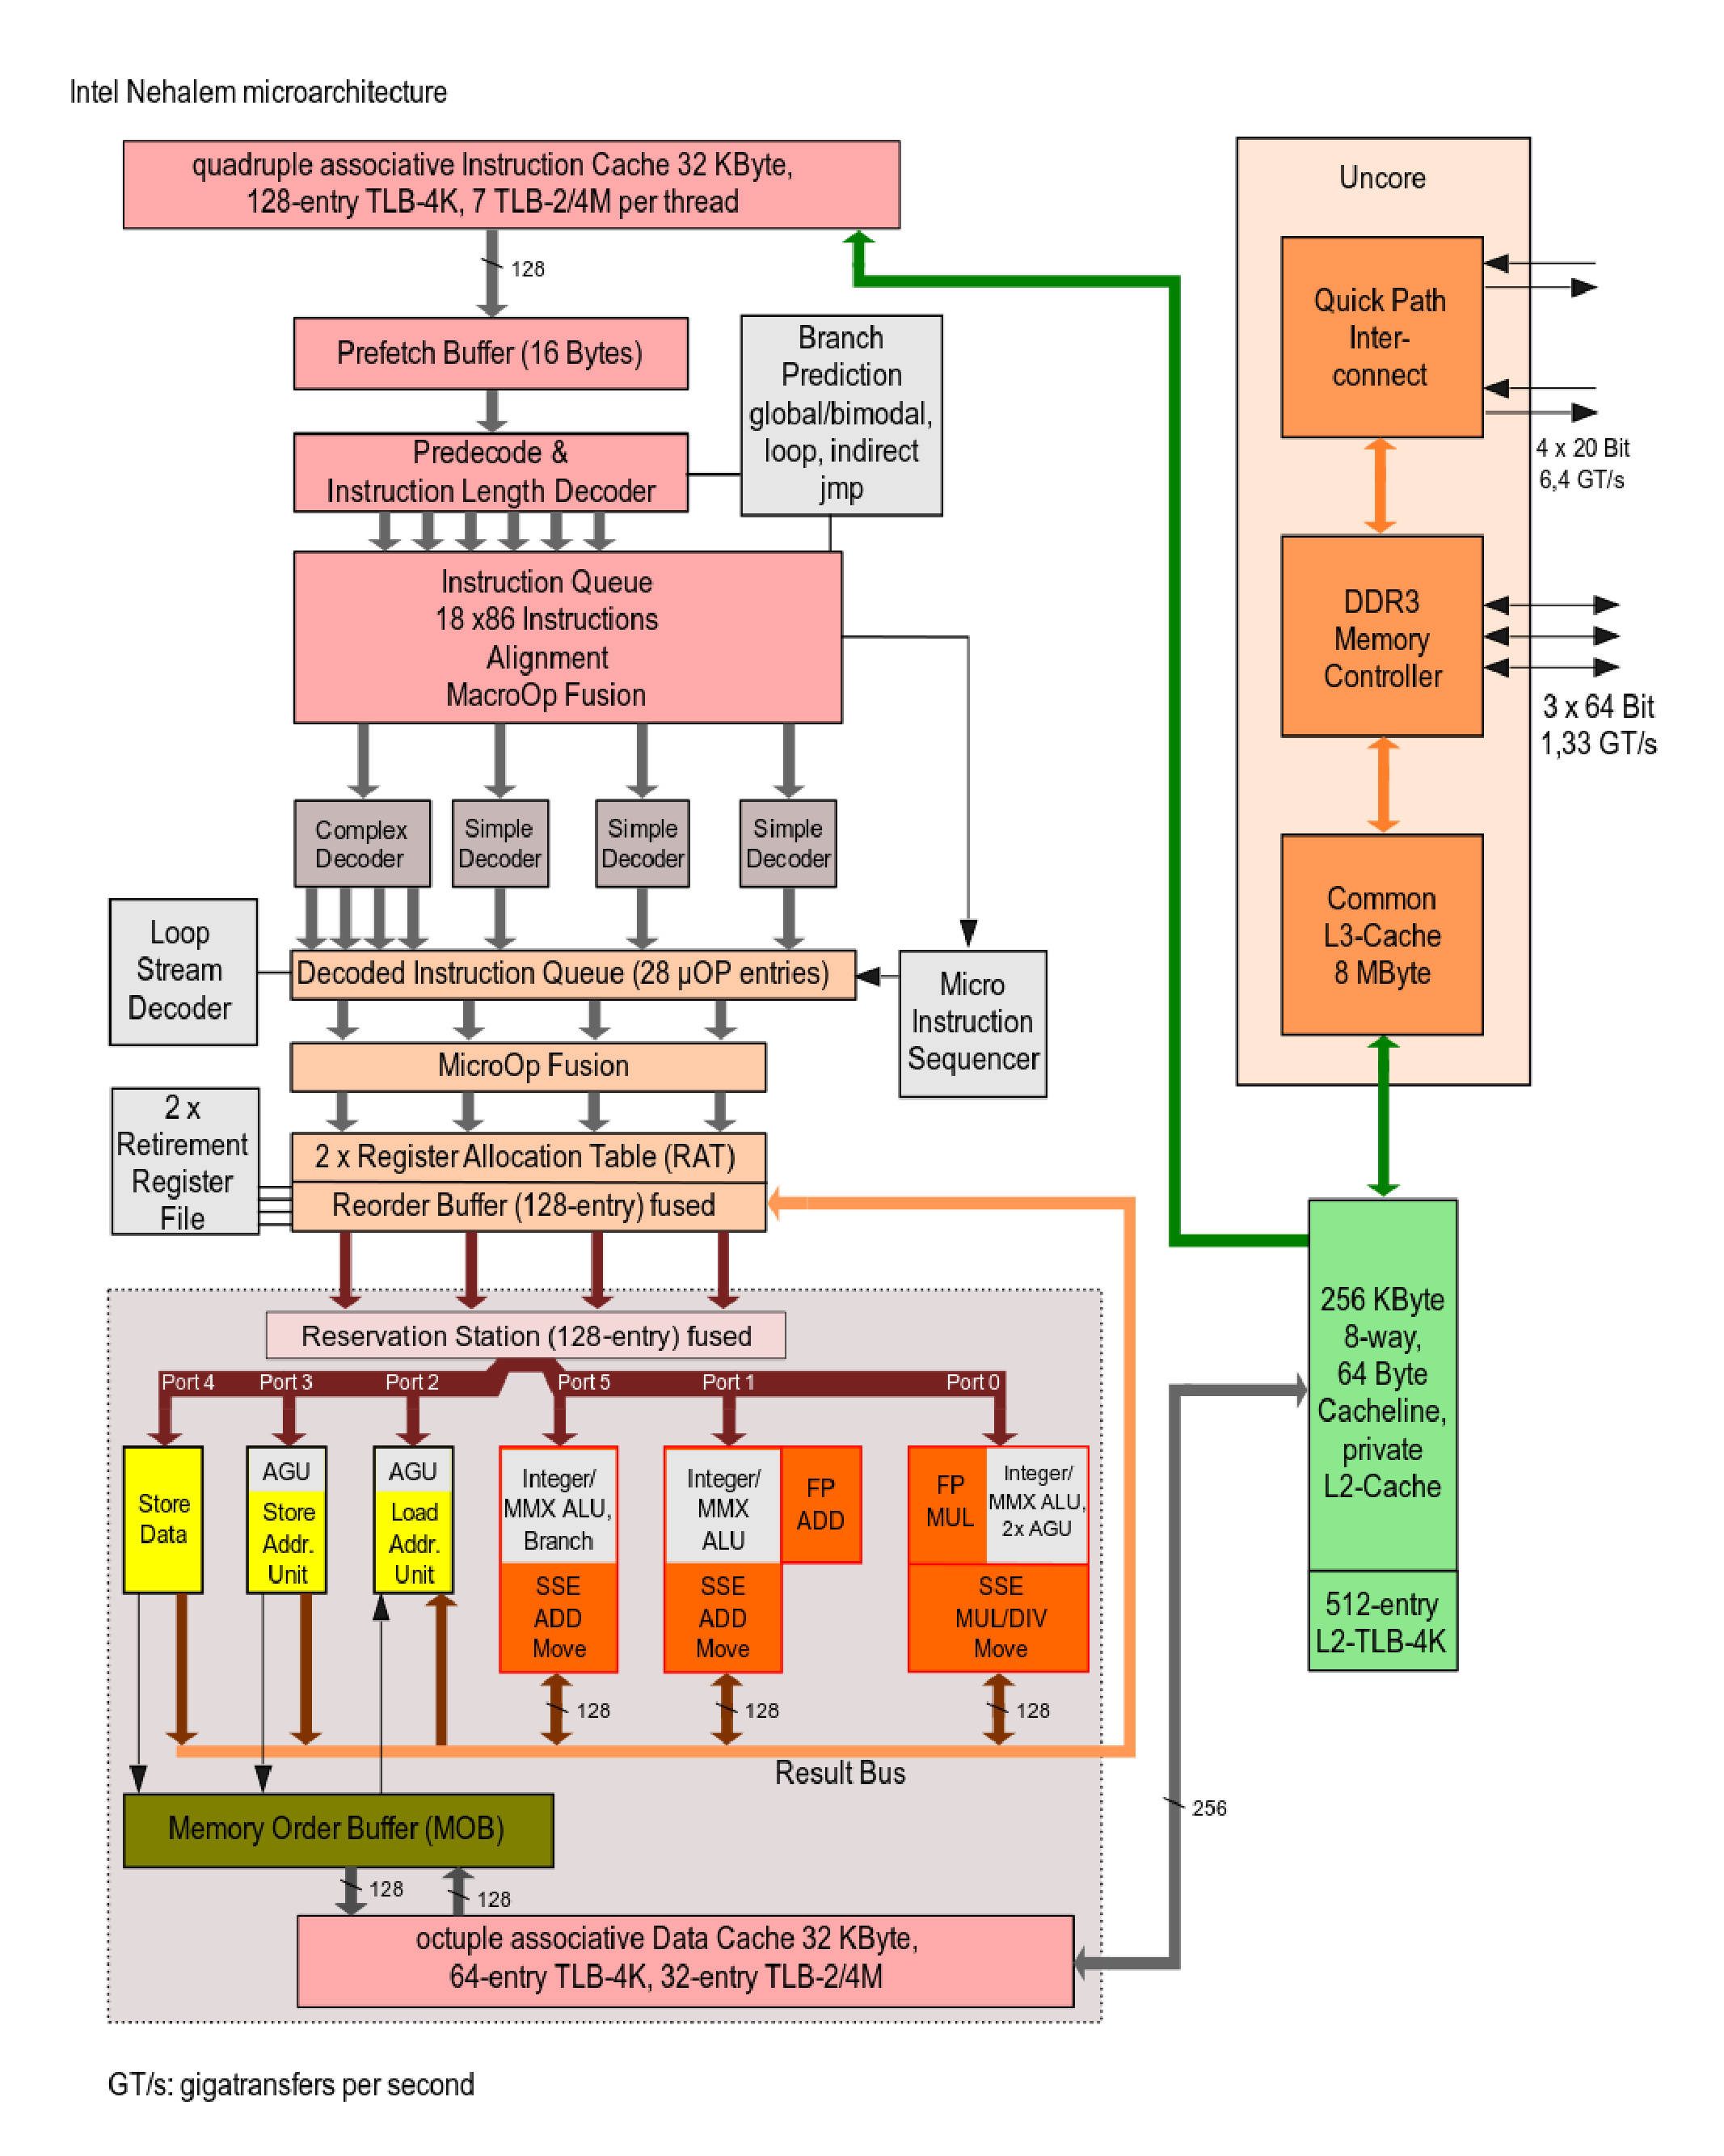
\includegraphics[width=0.6\textwidth]{nehalem_arch.pdf}}
  \end{center}
\end{frame}

\begin{frame}[fragile]{Out-of-order execution \& register renaming}
  \begin{tikzpicture}
    \node[text width=8cm]{
\begin{verbatim}
mov    eax, [rsp]
imul   eax, eax
mov    [rsp], eax
mov    eax, [rsp+0x4]
imul   eax, eax
mov    [rsp+0x4], eax
\end{verbatim}

will execute more similar to:

\begin{verbatim}
mov    eax0, [rsp]
mov    eax1, [rsp+0x4]
imul   eax0, eax0
imul   eax1, eax1
mov    [rsp], eax0
mov    [rsp+0x4], eax1
\end{verbatim}

    };
    \node at (4, 0) {
      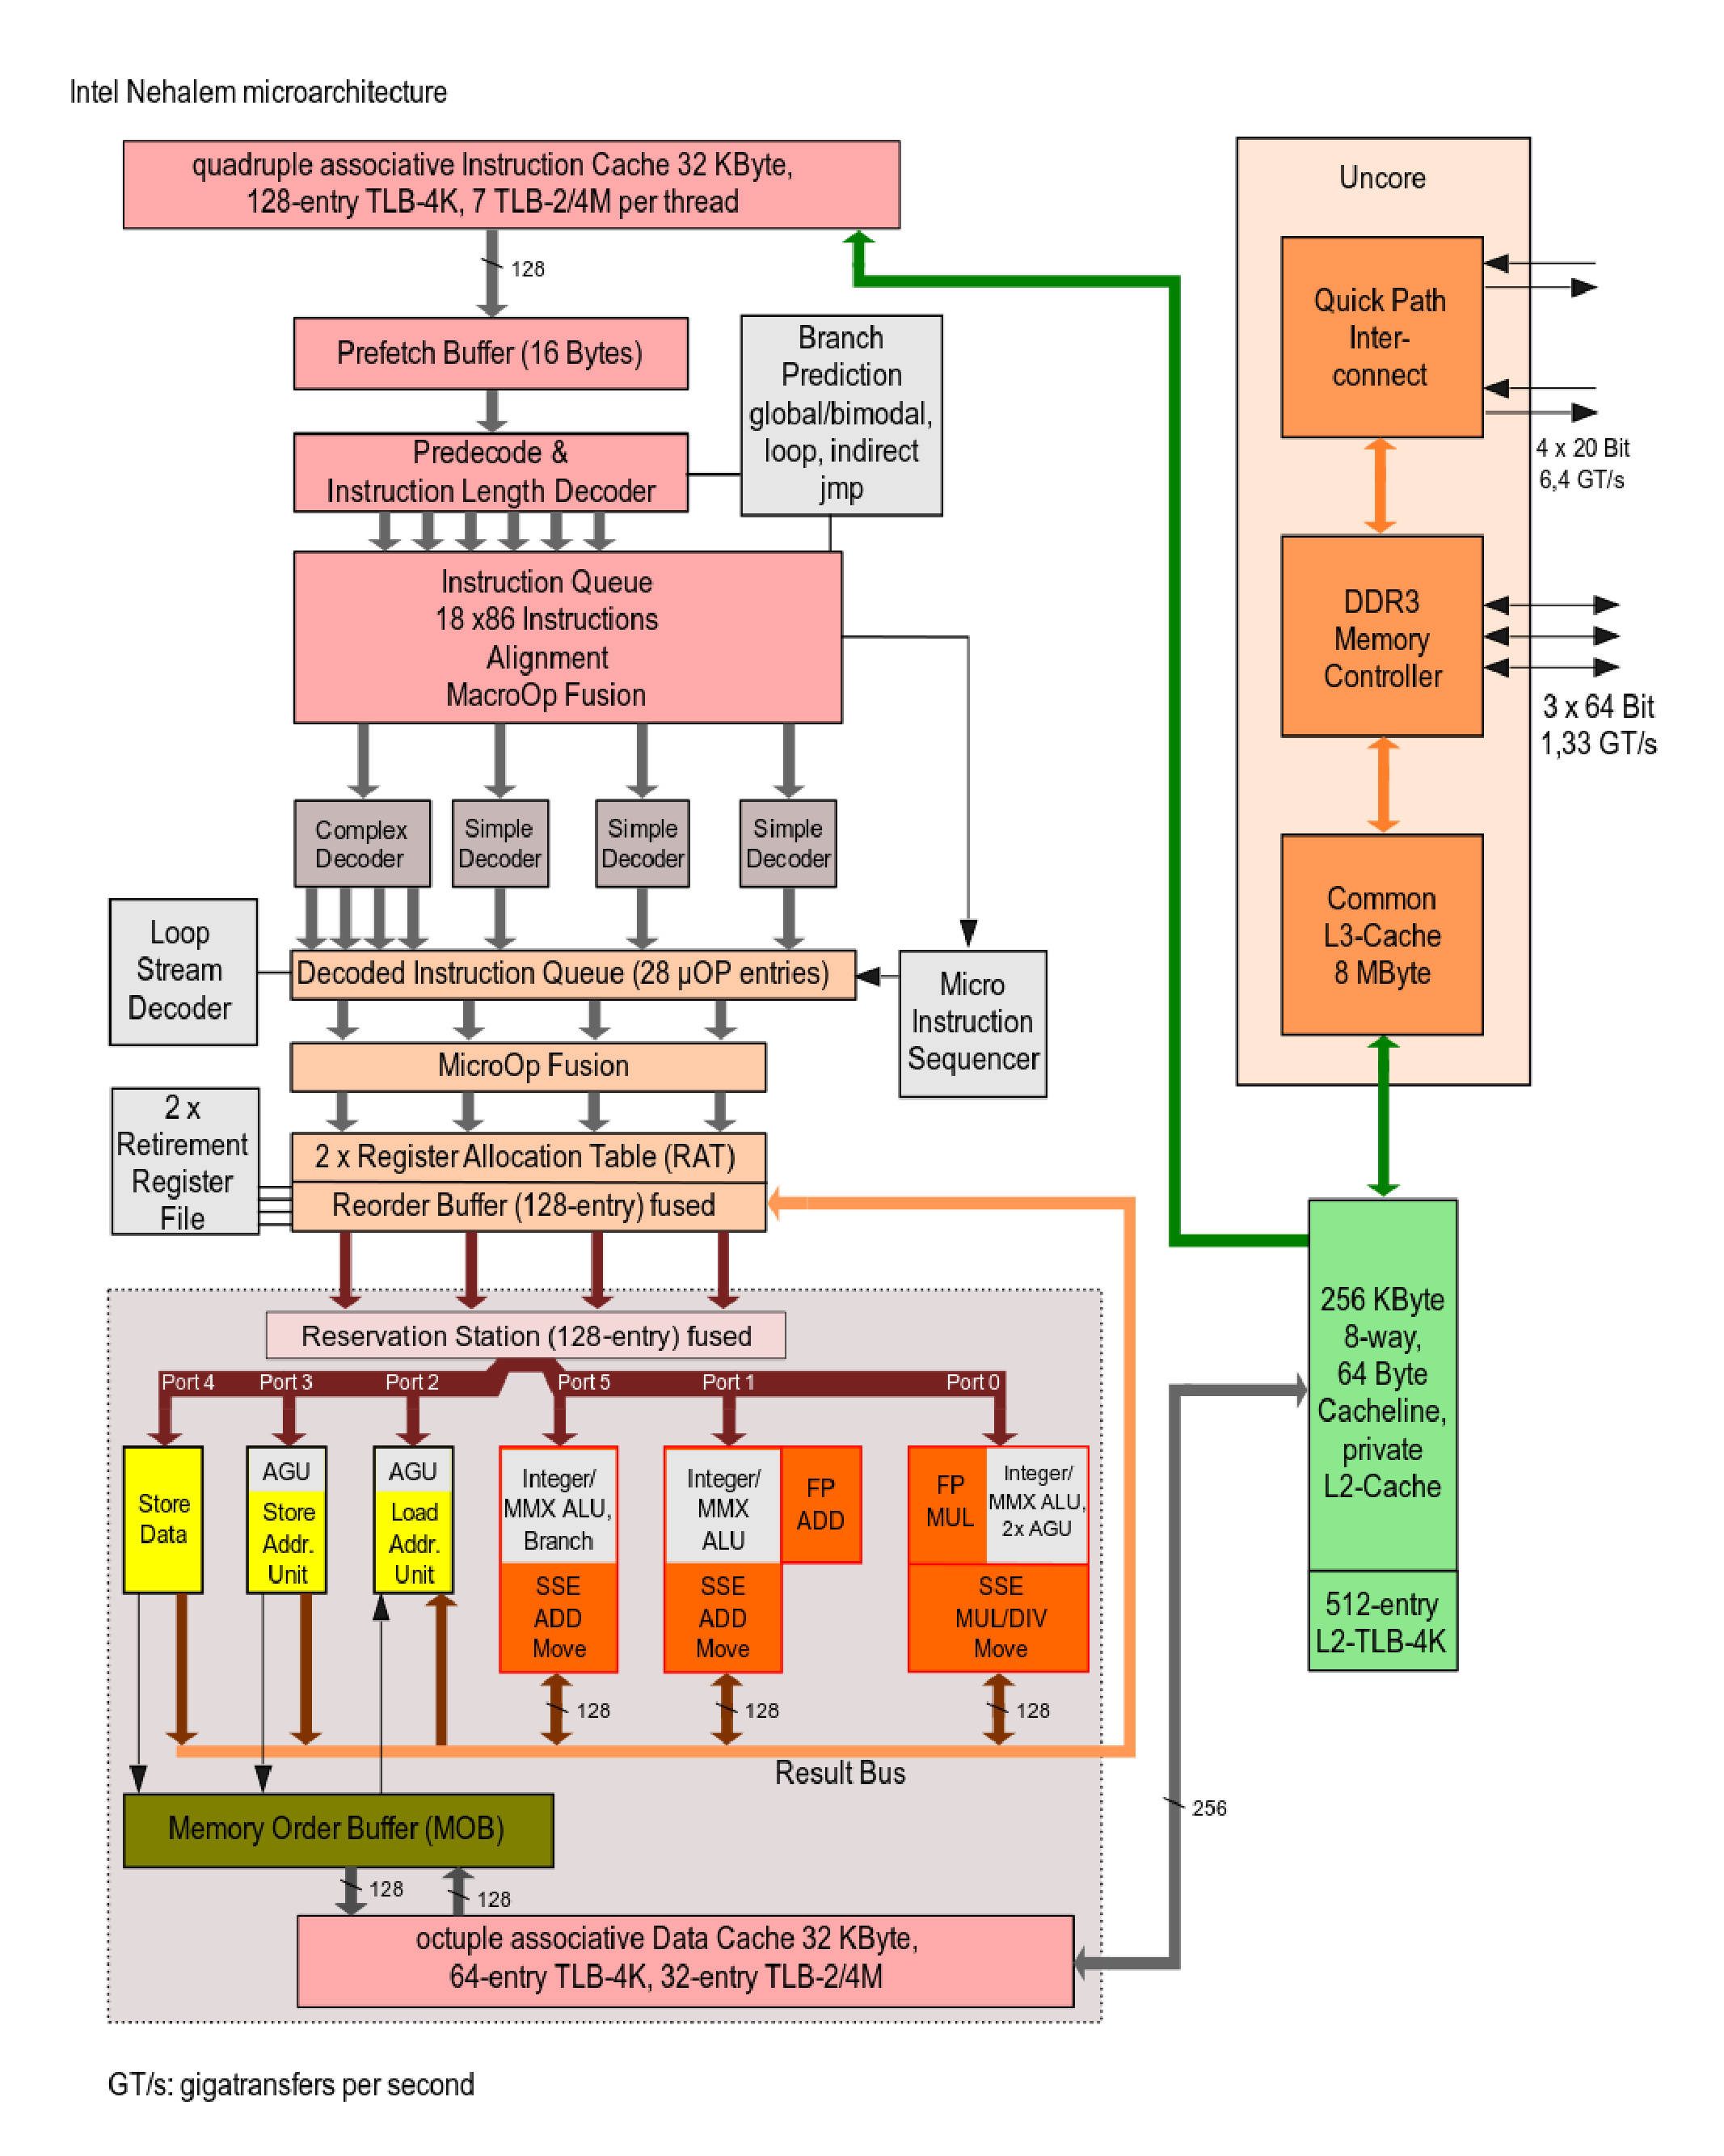
\includegraphics[width=0.6\textwidth]{nehalem_arch.pdf}
    };
  \end{tikzpicture}
\end{frame}

\begin{frame}[fragile]{Pipelining}
  \begin{tikzpicture}
    \node[text width=8cm]{
Not so good:
{\small
\begin{verbatim}
for (i = 2; i < n; ++i) {
    out[i] = a[i] * out[i - 2] + b[i] * out[i - 1];
}
\end{verbatim}
}

~

Good:
{\small
\begin{verbatim}
for (i = 0; i < n; ++i) {
    out[i] = a[i] + b[i];
}
\end{verbatim}
}
    };
    \node at (4.5, -3) {
      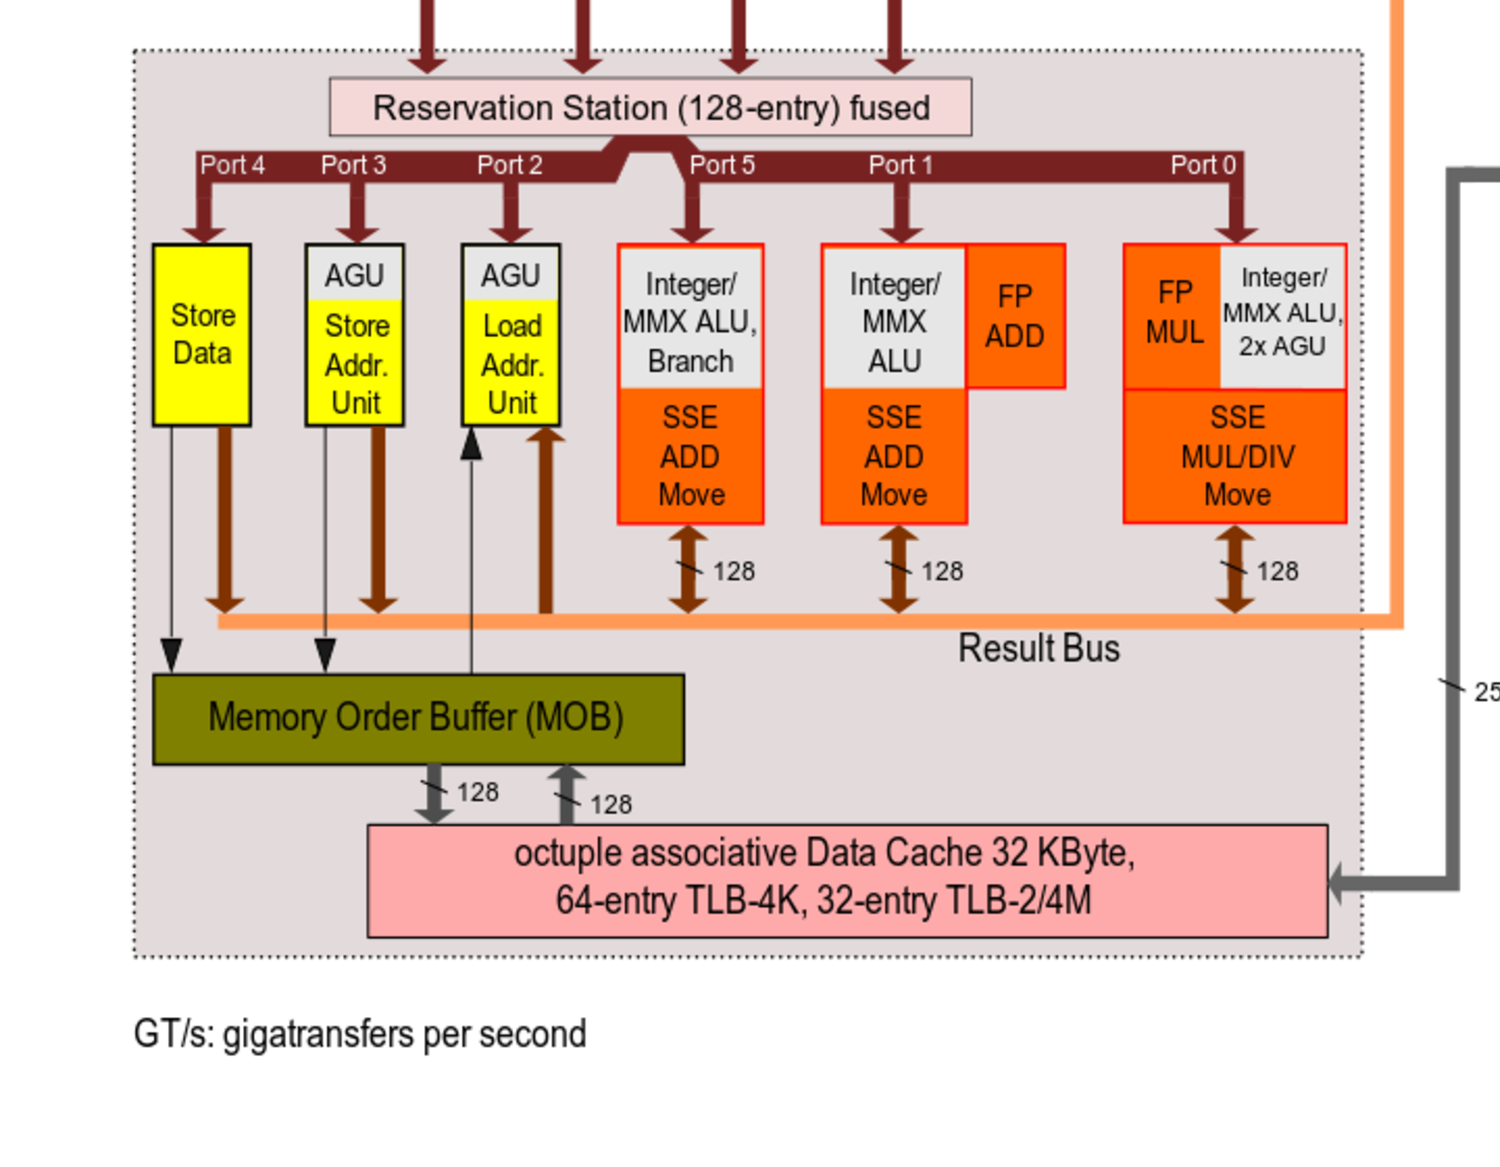
\includegraphics[width=0.7\textwidth]{nehalem_arch_crop.pdf}
    };
  \end{tikzpicture}
\end{frame}


\begin{frame}[fragile]{Branch prediction \& speculative execution}
  \begin{tikzpicture}
    \node[text width=8cm]{
\begin{verbatim}
x = f(y);
if (x < 100) {
    x *= 2;
} else {
   x -= 100;
}
\end{verbatim}
    };
    \node at (4.5, -3) {
      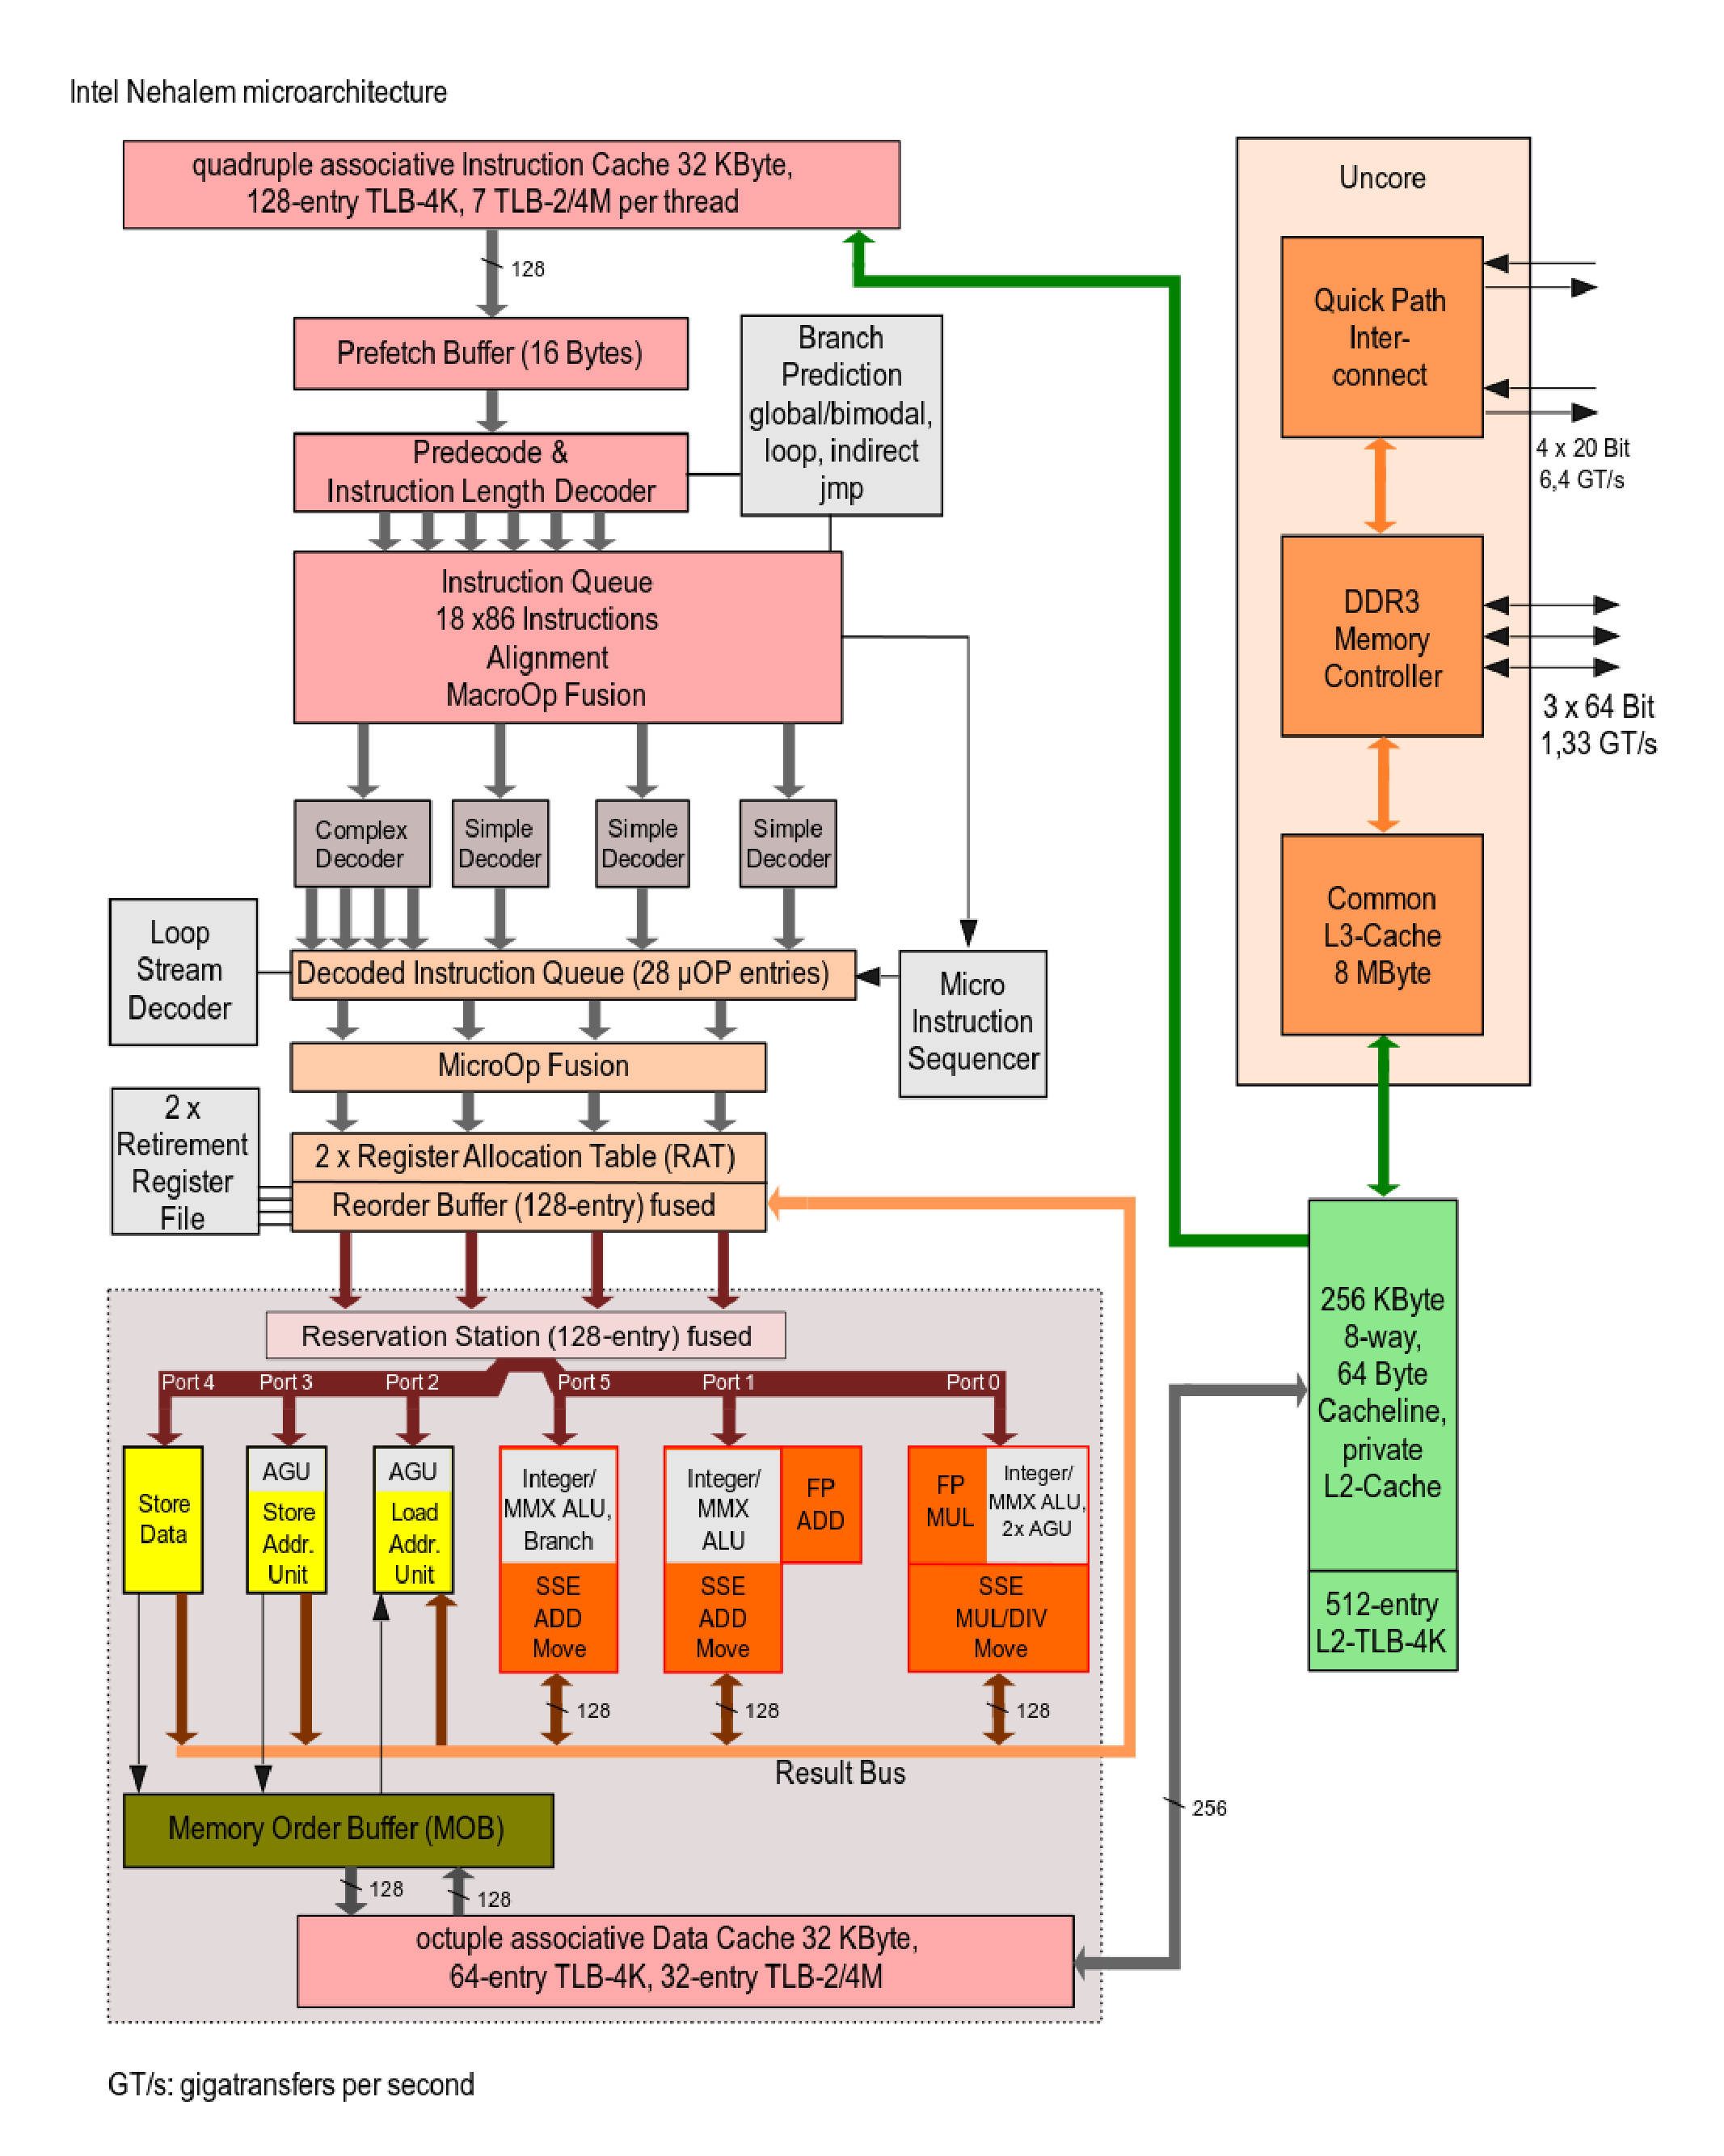
\includegraphics[width=0.6\textwidth]{nehalem_arch.pdf}
    };
  \end{tikzpicture}
\end{frame}

\begin{frame}{Vector instructions}
  \begin{itemize}
  \item SSE: 128-bit registers (4 $\times$ SP or 2 $\times$ DP)
  \item AVX: 256-bit registers (8 $\times$ SP or 4 $\times$ DP)
  \end{itemize}

~

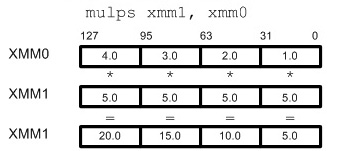
\includegraphics[width=.6\textwidth]{sse.jpg} 
\end{frame}

\end{document}